% useless experiment definitions
\paragraph{}
We mentioned in Section \ref{description_chapter} that the MersenneKEM cryptosystem is not guaranteed to always be correct. Instead, we claimed that it is correct with very high probability. In this chapter, we give experimental evidence to support this claim.

\theoremstyle{definition}
\begin{definition}{\textbf{Correctness of Cryptosystem}}
Let $(\mathcal{P}, \mathcal{C}, \mathcal{K}, \mathcal{E}, \mathcal{D})$ be a cryptosystem. We say the cryptosystem is correct if, for every $k \in \mathcal{K}$ and corresponding $e_k \in \mathcal{E}$ and $d_k \in \mathcal{D}$ the following holds:
\begin{align*}
    d_k \circ e_k &= id_\mathcal{P}\\
    e_k \circ d_k &= id_\mathcal{C}
\end{align*}
\end{definition}

\paragraph{}
In the decryption step of MersenneKEM, we used a heuristic to pick likely bits for the plaintext $(A, B)$. Unfortunately, due to the presence of this heuristic, it is not possible to guarantee that the cryptosystem is correct. We then turn so seeing if the cryptosystem is correct with high probability.

\theoremstyle{definition}
\begin{definition}{\textbf{Error Bound of Cryptosystem}}
Let $(\mathcal{P}, \mathcal{C}, \mathcal{K}, \mathcal{E}, \mathcal{D})$ be a cryptosystem. We say the cryptosystem has error bound $\epsilon$ if:
\begin{align*}
    Pr_{k \in \mathcal{K}} [d_k \circ e_k = id_\mathcal{P}] > 1 - \epsilon
\end{align*}
\end{definition}

\paragraph{}
We show that the error bound of MersenneKEM is very low for correct choices of cryptosystem parameters $n, h$ (defining $p = 2^n - 1$) and threshold parameter $\delta$, making it feasible in practice despite its correctness being unprovable.

% useless correctness "proof" from introduction
\subsection{Correctness}
\paragraph{}
As $A$ and $B$ both have Hamming weight $h$, we can regard them as bitstrings with one bits at exactly $h$ many points. Equivalently, we can write $A = 2^{a_1} + \dots + 2^{a_h}$ and $B = 2^{b_1} + \dots + 2^{b_h}$, where the $a_i$s are the indices of one bits in $A$ and $b_i$ are the indices of one bits in $B$. We then identify $A$ and $B$ with the sets $\alpha = \{ a_1, \dots, a_h \}$ and $\beta = \{ b_1, \dots, b_h \}$ respectively.

\paragraph{}
To see the likely correctness of the algorithm, we write $D = AF + BG$, as computed by Bob, as $2^{a_1} F + \dots + 2^{a_h} F + 2^{b_1} G + \dots + 2^{b_h}$. Then, by Lemma 2 of \cite{aggarwal2018new}, $Ham(D) - Ham(D - 2^{a_i} F) \leq Ham(2^{a_i} F)$ for each $a_i$ (and likewise for $G$ and the $b_i$s).

\paragraph{}
This inequality suggests that the Hamming weight reduction when subtracting some $2^i F$ or $2^j G$ from $D$ for choices of $i \in \alpha, j \in \beta$ could be very large, and we confirm experimentally that this is indeed the case for suitable choices of the parameters $n$ and $h$. We also confirm experimentally that when subtracting $2^i F$ or $2^j G$ from $D$ for choices of $i \not\in \alpha, j \not \in \beta$, the Hamming weight reduction is much smaller and may even be negative.

\paragraph{}
We can therefore have confidence that selecting a sets of bit indices $I$ and $J$ with Hamming weight decrease larger than a suitably chosen threshold $\delta$ as given above is likely to result in correct values of $A$ and $B$.

% old detailed description of cryptosystem
\paragraph{}
The key-exchange protocol assumes that Bob has generated his public-private key-pair and published his public key in a publicly-accessible database.

\paragraph{}
To compute his private key, Bob samples $F$ and $G$ uniformly and randomly from $\ham_h^n$. He then sets $(F, G)$ as his private key.

\paragraph{}
To compute his public key, Bob first computes $f = \mu(F) \in \F_p$ and $g = \mu(g) \in \F_p$. He then computes $h = f g^{-1}$ in the field $\F_p$ and then publishes $H = \mu^{-1}(h) \in \mathcal{B}_n$ as his public key.

\subsection{Encryption}
\paragraph{}
Alice randomly generates $A, B \in \ham_h^n$, together with the corresponding images $a = \mu(A), b = \mu(B)$ in $\F_p$. She then computes $c = a\mu(H) + b$ and sends $C = \mu^{-1}(c)$ to Bob.

\subsection{Decryption}
\paragraph{}
Bob receives $C$ from Alice and, using $G$ from his private key $(F, G)$, computes $d = \mu(C) \mu(G)$.

\paragraph{}
Bob first defines the following function:
\begin{align*}
\eta &: \F_p \times \Z_n \rightarrow \Z\\
\eta(s, i) &= Ham \circ \mu^{-1} (d) - Ham \circ \mu^{-1}(d - 2^i s)
\end{align*}

\paragraph{}
The result of computing $\eta(s, i)$ gives the amount that the Hamming weight of $d$ decreases by when subtracting $2^i s$ from it. This can be computed efficiently in $O(h)$.

\paragraph{}
Bob then computes the following sets:
\begin{align*}
I &= \{ i \in \Z_n : \eta(f, i) > \delta  \}\\
J &= \{ j \in \Z_n : \eta(g, j) > \delta  \}
\end{align*}

\paragraph{}
Bob then recovers the likely values of $A$ and $B$ in the following manner:
\begin{align*}
A &= \mu^{-1}(\sum_{i \in I} 2^i)\\
B &= \mu^{-1}(\sum_{j \in J} 2^j)
\end{align*}

The correctness of the decryption step hinges on the key claim that $I$ and $J$ contain the bits that are most likely to be set in $A$ and $B$ respectively. We make this claim more precise in Chapter \ref{correctness_chapter} and give bounds on the probability that this decryption step is incorrect.

\subsection{Key Extraction}

\section{Algorithmic Efficiency}

% threat models, perhaps move to preliminaries

\subsection{Threat Models}
\paragraph{}
Let $(\mathcal{P}, \mathcal{C}, \mathcal{K}, \mathcal{E}, \mathcal{D})$ be an instance of MersennePKC, with fixed parameters $n$ and $h$. Suppose Bob has a key $k = (F, G, H) \in \mathcal{K}$ (where $H$ is his public key) and that Alice is sending a plaintext $(A, B) \in \mathcal{P}$ to Bob We consider 2 threat models and how MersennePKC performs under them:
\begin{itemize}
    \item Chosen Plaintext Attack (CPA): The adversary attempts to learn information about $A, B, F, G$ while having access to an oracle $\mathcal{O}_k^\mathcal{E}: \mathcal{P} \rightarrow \mathcal{C}$ that takes plaintexts and outputs corresponding ciphertexts under the key $k$.
    \item Chosen Ciphtertext Attack (CCA): The adversary attempts to learn information about $A, B, F, G$ while having access to an oracle $\mathcal{O}_k^\mathcal{D}: \mathcal{C} \rightarrow \mathcal{P}$ that takes ciphertexts and outputs corresponding plaintexts under the key $k$.
\end{itemize}

\paragraph{}
Having defined the adversaries we are trying to defend against, we need to establish what it means to be secure against each of these adversaries. To do this, we use the notion of ciphertext indistinguishability.

\paragraph{}
Consider the following game between a probabilistic polynomial-time adversary and a (potentially unbounded) challenger:

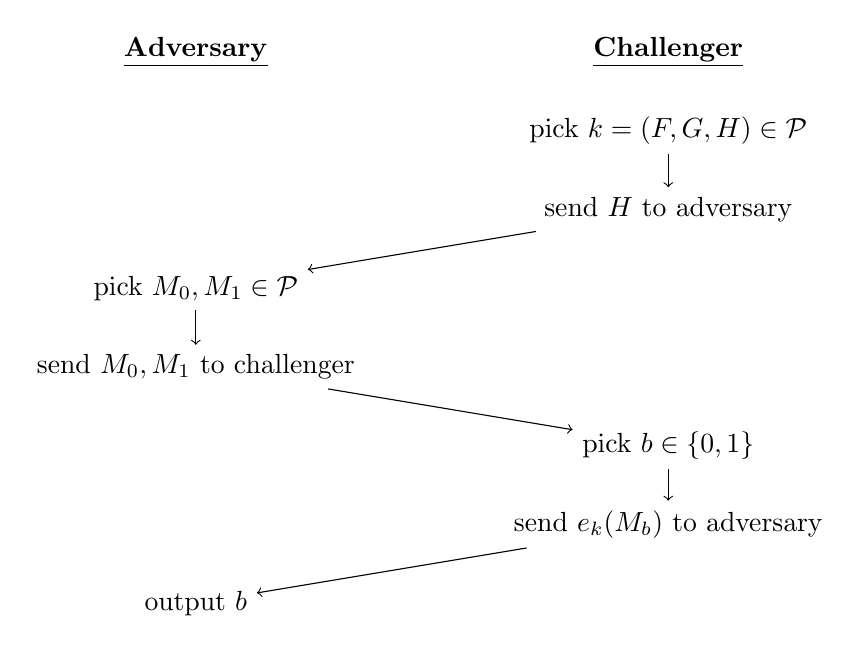
\begin{tikzpicture}
\node[] at (2, 51) {\underline{\textbf{Adversary}}};
\node[] at (8, 51) {\underline{\textbf{Challenger}}};
\node[](1) at (8, 50) {pick $k = (F, G, H) \in \mathcal{P}$};
\node[](2) at (8, 49) {send $H$ to adversary};
\node[](3) at (2, 48) {pick $M_0, M_1 \in \mathcal{P}$};
\node[](4) at (2, 47) {send $M_0, M_1$ to challenger};
\node[](5) at (8, 46) {pick $b \in \{0,1\}$};
\node[](6) at (8, 45) {send $e_k(M_b)$ to adversary};
\node[](7) at (2, 44) {output $b$};
\draw[->] (1) -- (2);
\draw[->] (2) -- (3);
\draw[->] (3) -- (4);
\draw[->] (4) -- (5);
\draw[->] (5) -- (6);
\draw[->] (6) -- (7);
\end{tikzpicture}

\paragraph{}
Let $\mathcal{Z}$ be the set of possible choices made by both the adversary and challenger in the game. Let $\mathcal{X}$ (resp. $\mathcal{Y}$)be the set of possible information available to the adversary in the case where the verifier chooses $b = 0$ (resp. $b = 1$).
\begin{align*}
\mathcal{Z} &= \{ ((F, G, H), M_0, M_1, b, C) \in \mathcal{K} \times \mathcal{P} \times \mathcal{P} \times \{0,1\} \times \mathcal{C} : C \in \{e_k(M_0), e_k(M_1)\} \}\\
\mathcal{X} &= \{ (H, M_0, M_1, C) : ((F, G, H), M_0, M_1, b, C) \in \mathcal{X}, b = 0\}\\
\mathcal{Y} &= \{ (H, M_0, M_1, C) : ((F, G, H), M_0, M_1, b, C) \in \mathcal{X}, b = 1\}\\
\end{align*}

\theoremstyle{definition}
\begin{definition}{\textbf{IND-CPA}}
We say that MersennePKC has the ciphertext indistinguishability under chosen plaintext attack (IND-CPA) if, for every probabilistic polynomial time adversary $\mathcal{A}$ the following holds:
\begin{align*}
    |\Pr_{x \in \mathcal{X}}[\mathcal{A}(x) = 1] - \Pr_{y \in \mathcal{Y}}[\mathcal{A}(y) = 1]| \in O(\frac{1}{2^h})
\end{align*}
\end{definition}

\theoremstyle{definition}
\begin{definition}{\textbf{IND-CCA}}
We say that MersennePKC has the ciphertext indistinguishability under chosen ciphertext attack (IND-CCA) if, for every probabilistic polynomial time adversary $\mathcal{A}$ allowed to make polynomially many queries to the decryption oracle $\mathcal{O}_k^\mathcal{E}$ (but not allowed to decrypt the given ciphertext),the following holds:
\begin{align*}
    |\Pr_{x \in \mathcal{X}}[\mathcal{A}(x) = 1] - \Pr_{y \in \mathcal{Y}}[\mathcal{A}(y) = 1]| \in O(\frac{1}{2^h})
\end{align*}
\end{definition}

\paragraph{}
\begin{figure}
\centering
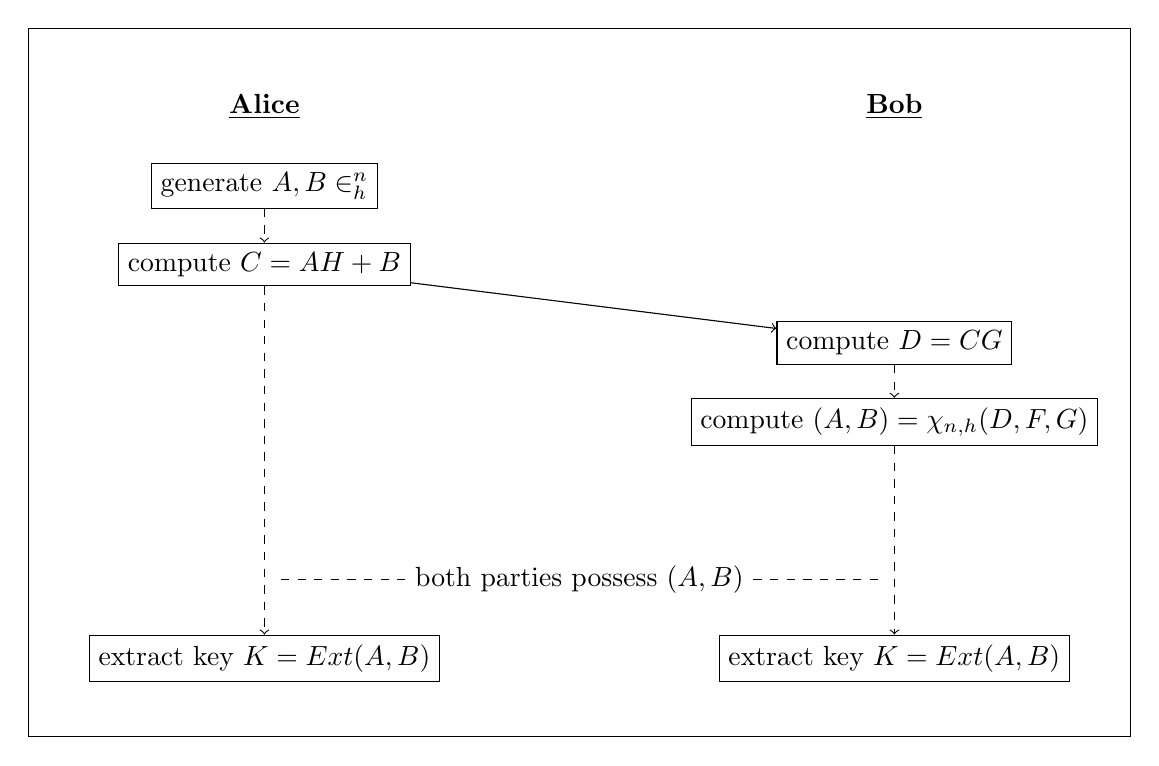
\begin{tikzpicture}
\node[draw](1) at (1,-1) {extract key $K = Ext(A,B)$};
\node[draw](2) at (9,-1) {extract key $K = Ext(A,B)$};
\node[draw](3) at (9,2) {compute $(A,B) = \chi_{n, h}(D, F, G)$};
\node[draw](4) at (9,3) {compute $D = CG$};
\node[draw](5) at (1,4) {compute $C = AH + B$};
\node[draw](6) at (1,5) {generate $A,B \in \ham_h^n$};
\node[](7) at (5, 0) {both parties possess $(A, B)$};
\node[](8) at (1, 0) {};
\node[](9) at (9, 0) {};
\node[] at (1,6) {\underline{\textbf{Alice}}};
\node[] at (9,6) {\underline{\textbf{Bob}}};
\draw[->] (5) -- (4);
\draw[dashed, ->] (6) -- (5);
\draw[dashed, ->] (5) -- (1);
\draw[dashed, ->] (4) -- (3);
\draw[dashed, ->] (3) -- (2);
\draw[dashed, -] (7) -- (8);
\draw[dashed, -] (7) -- (9);
\draw (-2,-2) rectangle (12,7);
\end{tikzpicture}
\caption{MersennePKC Protocol} \label{fig:M1}
\end{figure}

% CPA adversary

\paragraph{}
The semantic security of MersennePKC depends on 2 critical assumptions. The first is one that shows that it is difficult to recover the private key from the public key. The second is a modified version of a key assumption in \cite{aggarwal2018new}.

\paragraph{}
In the definition below, let $\mathcal{K}^c$ be the complement of $\mathcal{K}$ in $\ham_h^n \times \ham_h^n \times \mathcal{B}_n$.

\theoremstyle{definition}
\begin{definition}{\textbf{Mersenne Quotient Assumption}}
Given $F, G \in \ham_h^n$, $R \in \mathcal{U}(\mathcal{B}_n)$ and any probabilistic polynomial time Turing machine $\mathcal{A}$, we assume that:
\begin{align*}
    |\Pr_{(F, G, H) \in \mathcal{K}}[\mathcal{A}(\frac{F}{G}) = 1] - \Pr_{(F, G, R) \in \mathcal{K}^c}[\mathcal{A}(R) = 1]| \in O(\frac{1}{2^n})
\end{align*}
\end{definition}

\paragraph{}
The Mersenne quotient assumption ensures that, for some key $(F, G, \frac{F}{G}) \in \mathcal{K}$, a probablistic polynomial time adversary cannot obtain any information about the private key $(F, G)$ given only the public key $\frac{F}{G}$.

\theoremstyle{definition}
\begin{definition}{\textbf{Mersenne Low Hamming Combination}}
Given $n, h \in \N$ where $p = 2^n - 1$ is a Mersenne prime and $n > 2h^2$, any probabilistic polynomial time adversary attempting to distinguish $(H, AH + B)$ and $(H, R)$ is at most $O(\frac{1}{2^h})$, where $H, R \sim \mathcal{U}(\mathcal{B}_n)$ and $A, B \in \ham_h^n$.
\end{definition}


% waffling, maybe put in conclusion
\section{Post-Quantum Cryptosystems}
\paragraph{}
In light of various breakthroughs in producing quantum computers, several new cryptosystems based on problems thought to be hard even on quantum computers have been proposed. One such example is lattice-based cryptosystems such as Learning with Errors \cite{regev2009lattices}, based on the supposed hardness of finding the approximate shortest nonzero vector in a lattice. While lattice-based cryptosystems are popular, nothing precludes the possiblity of an efficient quantum algorithm being discovered in the future breaking them. Therefore, a key exchange protocol based on a different hardness assumption, the Mersenne Low Hamming Combination Assumption, was proposed in \cite{aggarwal2018new}.



Let $+: \mathcal{B}_n \rightarrow \mathcal{B}_n$ be the function performed by the following algorithm:
\begin{lstlisting}[mathescape=true]
ADD($a$, $b$):
    c := BITWISE-ADD-WITH-CARRY($a_n \dots a_1$, $b_n \dots b_1$)
    d := BITWISE-ADD-WITH-CARRY($c_n \dots c_1$ and $0^{n-1} c_{n+1}$)
    return d
\end{lstlisting}

% sufficiency lemma
\subsection{Sufficiency of Two Iterations}
\textbf{TODO: Make this a lemma and maybe move it to preliminaries.}
\paragraph{}
Assuming the first and second iteration hypotheses hold, for each repetition $\iota$ we have picked two sets $U_\iota$ and $U_\iota'$, each of which is a subset of $\alpha_\iota$. It also holds that $U_\iota \cap U_\iota' = \emptyset$ with high probability by the second iteration hypothesis, since a point $i \in U_\iota \cap U_\iota'$ is considered an erroneous point in the second iteration.

\paragraph{}
Given that the two iteration hypotheses hold, we have that $U_\iota \cup U_\iota' \subseteq \alpha_\iota$. We now hypothesise that, with high probability, $U_\iota \cup U_\iota' = \alpha_\iota$.

\paragraph{\textbf{Sufficiency Hypothesis}} Let $Z \sim N(\mu_{\mathcal{I}'}, \sigma_{\mathcal{I}'}^2)$.
We hypothesise that $Pr[Z \leq \mu_{\mathcal{I}'} - 5 \sigma_{\mathcal{I}'}]$ is small.

% semantic security in intro... trash
\subsection{Semantic Security}
\paragraph{}
We note that the only data sent across the insecure channel is $A \frac{F}{G} + B$.

\paragraph{}
Suppose $A, B \in \ham_h^n$ are uniformly and randomly chosen. The cryptosystem relies on the assumption that the tuples $(\frac{F}{G}, A \frac{F}{G} + B)$ and $(\frac{F}{G}, R)$ for arbitrary $R \in \F_2^n$ are computationally indistinguishable for a probabilistic polynomial-time adversary. In particular, we assume that the adversary can distinguish the two with probability at most $O(2^{-h})$, this making $h$ the security parameter.

\paragraph{}
This assumption is given as the Mersenne Low Hamming Combination Assumption in Definition 5 of \cite{aggarwal2018new}, but we state it here in a more specific and modified from to account for the fact the cryptosystem presented here is slightly different.